\documentclass[12pt,a4paper]{article}

\usepackage[brazil]{babel}
\usepackage[export]{adjustbox}
\usepackage[utf8]{inputenc}
\usepackage{graphicx}

\graphicspath{ {./img/} }

\title{Instruções de Uso do Componente PDF para Prisma}
\author{Douglas Rodrigues de Almeida}
\date{04 de Agosto de 2018}

\begin{document}

\maketitle

\section{Introdução}
O Componente PDF para Prisma é uma ferramenta para auxiliar a geração de documentos eletrônicos em PDF a partir da solicitação de impressão realizada no sistema Prisma.

\section{Configurando o Prisma}
Após a instalação do componente, é necessário configurar o Prisma para gerar arquivos em PDF. Essa configuração é individual, sendo registrada na matrícula do servidor. Portanto, só deve ser feita uma única vez, ainda que o usuário mude de computador.

\subsection{Para configurar sua matrícula no Prisma para gerar PDF:}
1. Abra o Prisma clicando no seu ícone na área de trabalho.

2. Autentique-se com sua matrícula e senha.

\pagebreak
3. No menu principal, vá para BENEFÍCIOS.\\
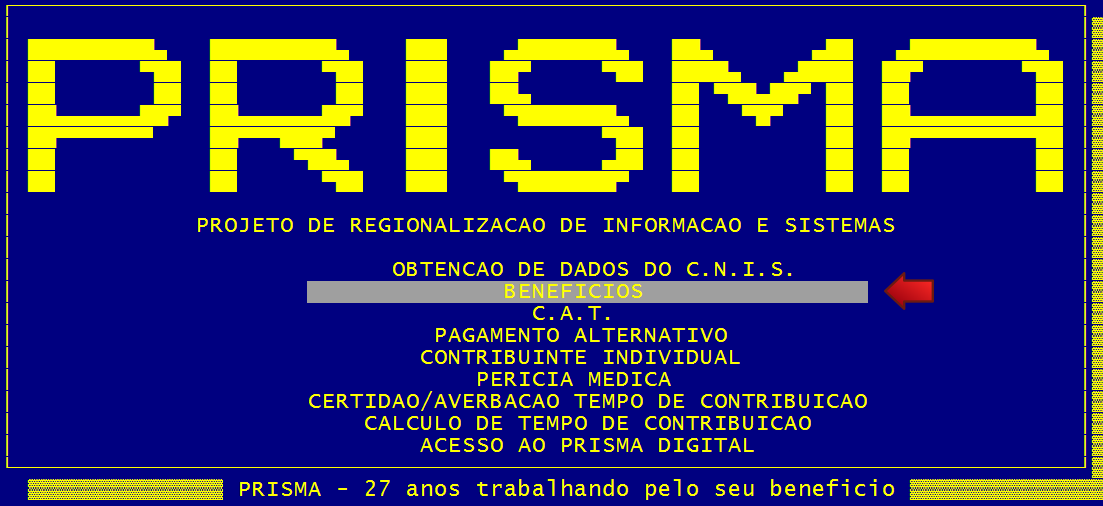
\includegraphics[width=1.0\textwidth, center]{menu}\\

\vspace{0.3cm}
4. Na tela Benefícios, pressione a tecla *.\\
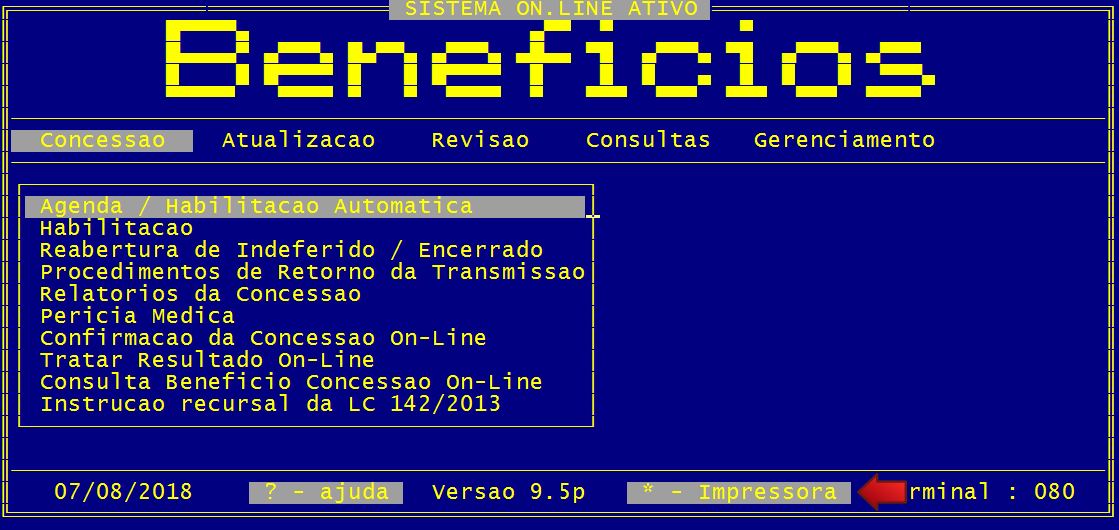
\includegraphics[width=1.0\textwidth, center]{beneficios}\\

\pagebreak
5. Na tela Cadastro da Impressora Padrão, pressione a tecla M seguida de ENTER.\\
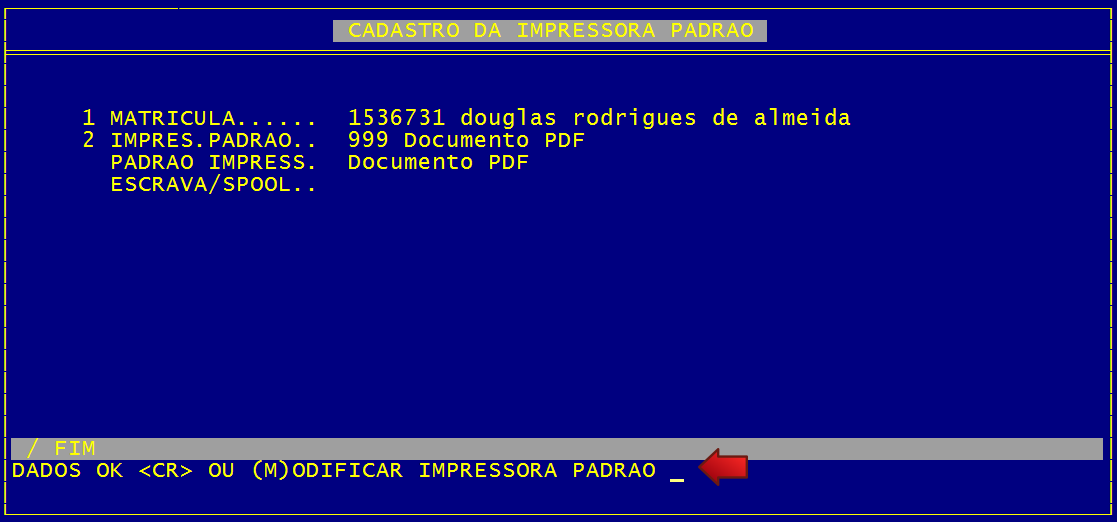
\includegraphics[width=1.0\textwidth, center]{modimpressora}\\

\vspace{0.3cm}
6. Em seguida, pressione a tecla ? seguida de ENTER.

7. Na lista de impressoras, escolha Documento PDF e pressione ENTER duas vezes.\\
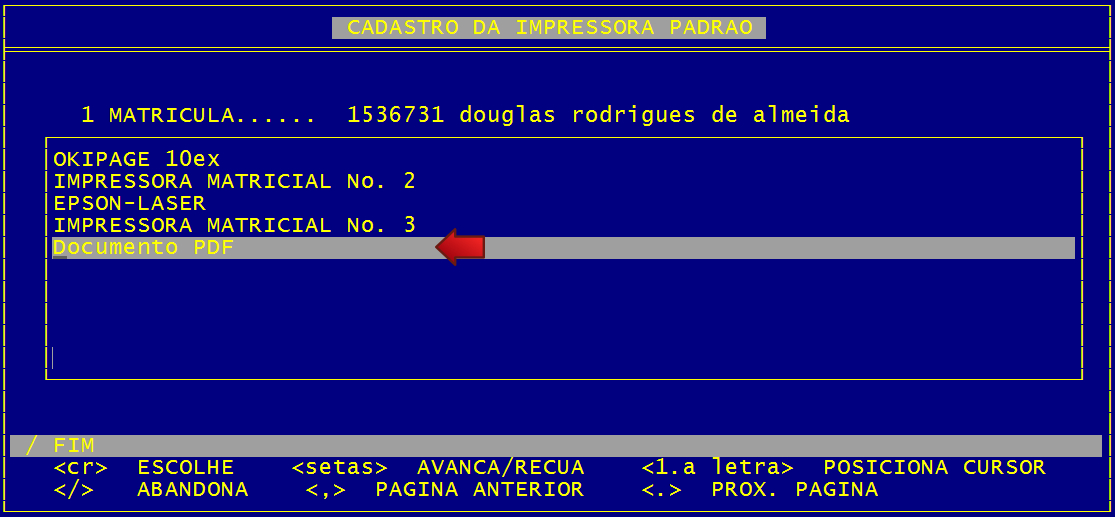
\includegraphics[width=1.0\textwidth, center]{listaimpressoras}\\

\vspace{0.3cm}
\noindent Uma vez configurado para gerar arquivos PDF a partir da impressão de relatórios, é possível desfazer essa alteração para voltar a impressão em papel físico.

\subsection{Para configurar sua matrícula para imprimir em papel físico:}
\begin{enumerate}
  \item Abra o Prisma clicando no seu ícone na área de trabalho.
  \item Autentique-se com sua matrícula e senha.
  \item No menu principal, vá para BENEFÍCIOS.
  \item Na tela Benefícios, pressione a tecla *.
  \item Na tela Cadastro da Impressora Padrão, pressione a tecla M seguida de ENTER.
  \item Em seguida, pressione a tecla ? seguida de ENTER.
  \item Na lista de impressoras, escolha LASERJET/CORREA e pressione ENTER duas vezes.
\end{enumerate}

\section{Problemas encontrados}
\begin{itemize}
  \item Nem todos os relatórios do Prisma são compatíveis com a geração de PDFs. Ao gerar um relatório incompatível, nada acontece. A correção desse problema somente ocorrerá em futuras versões do Prisma.
\end{itemize}

\end{document}
